\chapter{Charged current weak interactions}

The theory was originally developed by Fermi in the 1930s and his coupling constant $G_F$, from 1934, described weak interactions.  This developed from a pointlike theory to being mediated via a vector boson with coupling constant $g_{\mu\nu}$.

Consider the leptonic processes:

\begin{eqnarray*}
  \mu^+ & \to & e^+ \quad \nu_e \quad \bar{\nu}_{\mu} \\
  \nu_{\mu} \quad \e & \to & \mu^- \nu_e
\end{eqnarray*}

Fermi would have considered these reactions to be pointlike interactions between vector currents.

\begin{figure}[!htb]
  \begin{center}
    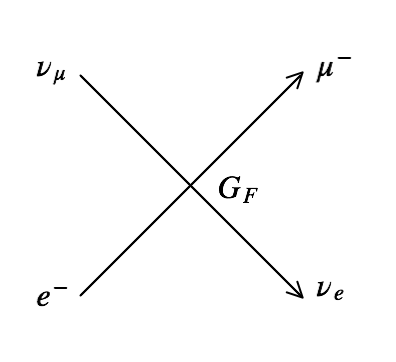
\includegraphics[width=0.5\textwidth]{images/web_feynman/image_42.png}
    \caption[Fermi picture of scattering]{Fermi picture of scattering.}
    \label{fig:ch12_FermiScattering}
  \end{center}
\end{figure}

This theory was modelled on the electromagnetic interaction but without the exchanged particle because the range of the weak force was known to be small.

Fermi suggested the following:

\[
  T_{fi} = G_F\bar{u}_{\mu^-}\gamma^{\mu}u_{\nu_{\mu}}\bar{u}_{\nu_{e}}\gamma_{\mu}u_{e^-}
\]

Now $G_F$ can be determined by experiment eg by measuring the muon (or some nuclear beta) decay rate.

\[
  Rate = |T_{fi}|^2 \times \textrm{ external factors}
\]

Parity violation was discovered in 1956, which meant that the weak current had to be modified from vector to vector-axial vector currents.

The transition probability reads:

\[
  T_{fi} = \frac{G_F}{\sqrt{2}}\bar{u}_{\mu^-}\gamma^{\mu}(1 - \gamma^5)u_{\nu_{\mu}}\bar{u}_{\nu_e}\gamma_{\mu}(1 - \gamma^5)u_{e^-}
\]

Presently the known form of the charged current weak interaction is different to the diagram given above.

\begin{figure}[!htb]
  \begin{center}
    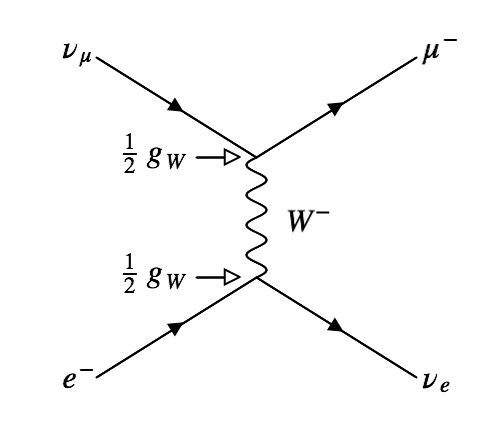
\includegraphics[width=0.5\textwidth]{images/web_feynman/image_43.png}
    \caption[Charged current scattering]{Charged current scattering.}
    \label{fig:ch12_chargedCurrentScattering}
  \end{center}
\end{figure}

\begin{eqnarray*}
  T_{fi} & = & \bar{u}_{\mu^-}\frac{\gamma^{\mu}}{2}(1 - \gamma^5)u_{\nu_{\mu}}\left(\frac{-g_W}{\sqrt{2}}\right)\frac{-g_{\mu\nu} + \frac{q_{\mu}q_{\nu}}{M_W^2}}{q^2 - M_W^2}\left(\frac{g_W}{\sqrt{2}}\right)\bar{u}_{\nu_e}\frac{\gamma_{\mu}}{2}(1 - \gamma^5)u_{e^-} \\
  & = & \bar{u}_{\mu^-}\gamma^{\mu}(1 - \gamma^5)u_{\nu_{\mu}}\frac{g_W^2}{4}\left(\frac{-g_{\mu\nu} + \frac{q_{\mu}q_{\nu}}{M_W^2}}{q^2 - M_W^2}\right)\bar{u}_{\nu_e}\gamma_{\mu}(1 - \gamma^5)u_{e^-}
\end{eqnarray*}

Comparing the old and new description for $|T_{fi}|^2$ in the limit $q^2/M_W^2 \to 0$:

\begin{eqnarray*}
  \frac{G_F^2}{2} & = & \left(\frac{1}{2}\frac{g_W}{\sqrt{2}}\frac{1}{M_W^2}\frac{g_W}{\sqrt{2}}\frac{1}{2}\right)^2 \\
  & = & \frac{g_W^4}{64M_W^4} \\
  \Rightarrow \frac{G_F}{\sqrt{2}} & = & \frac{g_W^2}{8M_W^2}
\end{eqnarray*}

The chiral doublet is:

\[
  \left(
    \begin{array}{c}
    \nu_{e} \\
    e^-
    \end{array}
  \right)_L
  = \frac{1}{2}\left(1 - \gamma_5\right)
  \left(
    \begin{array}{c}
    \nu_{e} \\
    e^-
    \end{array}
  \right)
\]

The right-handed singlet is:

\[
  e^-_R = \frac{1}{2}\left(1 + \gamma_5\right)e^-
\]

In $SU(2)\otimes U(1)$ electroweak unification fundamental entities are left-handed chiral doublets and right-handed singlets in weak isospin space.  The charged current weak interaction is of the form $\bar{u}_L\gamma^{\mu}u_L$:

\begin{eqnarray*}
  \left(\frac{1}{2}\left(1 - \gamma^5\right)\right)^2 & = & \frac{1}{4}\left(1 - 2\gamma^5 + \left(\gamma^5\right)^2\right) \\
  & = & \frac{1}{2}\left(1 - \gamma^5\right) \\
  \Rightarrow \bar{U}_e \frac{1}{2}\gamma^{\mu}\left(1 - \gamma^5\right)U_{\nu_e} & = & \bar{U}_e \gamma^{\mu}\left(\frac{1 - \gamma^5}{2}\right)^2U_{\nu_e} \\
  & = & \bar{U}_e \left(\frac{1 + \gamma^5}{2}\right)\gamma^{\mu}\left(\frac{1 - \gamma^5}{2}\right)U_{\nu_e} \\
  \Rightarrow \bar{U}_{eL} & = & \bar{U}_e\left(\frac{1 + \gamma^5}{2}\right) \\
  U_{\nu_eL} & = & \left(\frac{1 - \gamma^5}{2}\right)U_{\nu_e}
\end{eqnarray*}

So the charged current can be written as $\bar{U}_L \gamma^{\mu}U_L$.  By convention, $U_L$ will be taken to mean $\left(\begin{array}{c}\nu_e\\ \e^-\end{array}\right)_L$.

\section{Leptonic charge current process}

\begin{itemize}
  \item Muon decay has been exhaustively studied theoretically and experimentally since the late 1940s.
  \item It is possible to calculate the charged current weak interaction contribution to $\nu_e e$ scattering.  With small modifications this will apply to $\nu_e / \bar{\nu}_e q$ scattering.  The calculation is given here for $q^2 \ll M_W^2$ ie $W$ propagator effects can be neglected.  In fact $\nu$ experiments have not been in a high enough energy range to see any $W$ propagator effects.  However, the processes have been observed at HERA through the process $e^- q \to \nu q'$.  Effects have been seen for $M_W^2 \simeq 10^4 \gev^2$
\end{itemize}

\begin{figure}[!htb]
  \begin{center}
    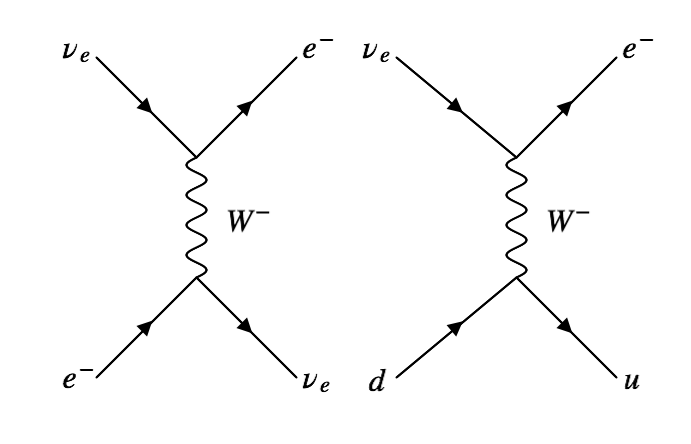
\includegraphics[width=0.8\textwidth]{images/web_feynman/image_44.png}
    \caption[Charged current interaction]{Charged current interaction.}
    \label{fig:ch12_chargedCurrentInteraction}
  \end{center}
\end{figure}

\begin{figure}[!htb]
  \begin{center}
    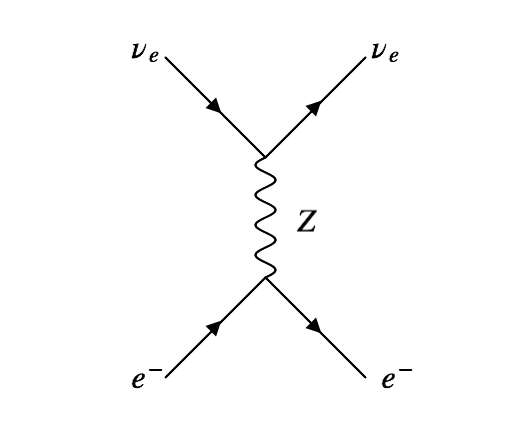
\includegraphics[width=0.6\textwidth]{images/web_feynman/image_45.png}
    \caption[Neutral current interaction]{Neutral current interaction.}
    \label{fig:ch12_neutralCurrentInteraction}
  \end{center}
\end{figure}

In the point-like limit:

\begin{figure}[!htb]
  \begin{center}
    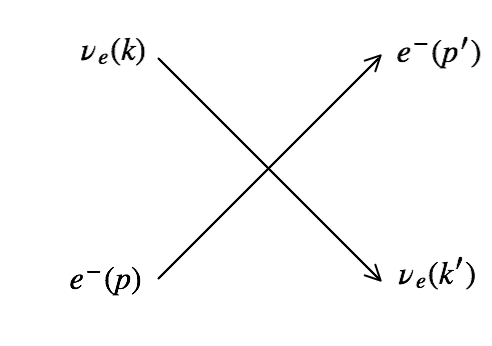
\includegraphics[width=0.5\textwidth]{images/web_feynman/image_46.png}
    \caption[Point-like charged current interaction]{Point-like charged current interaction.}
    \label{fig:ch12_chargedCurrentInteractionPointlike}
  \end{center}
\end{figure}

\[
  T_{fi} = \frac{G_F}{\sqrt{2}}\bar{u}(p')\gamma^{\mu}\left(1 - \gamma^5\right)u(k)\bar{u}(k')\gamma_{\gamma}\left(1 - \gamma^{\mu}\right)u(p)
\]

As usual it is necessary to find $T_{fi}^* T_{fi} = T_{fi}^{\dagger}T_{fi}$ summed over all spins and averaged over initial spins.

For the Hermitian conjugate consider one term:

\begin{eqnarray*}
  \Big[ \bar{u}(k')\gamma_{\mu}\left(1 - \gamma_5\right) u(p)\Big]^{\dagger} & = & u^{\dagger}(p)\left(1 - \gamma^5\right)^{\dagger}\gamma_{\mu}^{\dagger}\gamma_0^{\dagger}u(k') \\
  \textrm{as } \bar{u}(k') & = & u(k)\gamma_0
\end{eqnarray*}

Take $\gamma_{\mu} = \gamma_0$ or $\gamma_{\mu} = \gamma_k$.

Recall $\left(\gamma^0\right)^{\dagger} = \gamma^0 \quad \left(\gamma^5\right)^{\dagger} = \gamma^5 \quad \left(\gamma^k\right)^{\dagger} = -\gamma^k$

\paragraph{i} For $\gamma^{\mu} = \gamma^0$ the expression now reads:

\begin{eqnarray*}
  && u^{\dagger}(p)\left(1 - \gamma^5\right)\gamma_0\gamma_0u(k') \\
  & = & -u^{\dagger}(p)\gamma_0\left(1 - \gamma^5\right)\gamma_0u(k') \\
  & = & u^{\dagger}(p)\gamma_0\gamma_0\left(1 - \gamma^5\right)u(k') \\
  & = & \bar{u}(p)\gamma_0\left(1 - \gamma^5\right)u(k')
\end{eqnarray*}

\paragraph{ii} For $\gamma^{\mu} = \gamma^{k}$ the expression now reads:

\begin{eqnarray*}
  && u^{\dagger}(p)\left(1 - \gamma^5\right)\left(-\gamma_k\right)\gamma_0u(k') \\
  & = & -u^{\dagger}(p)(-\gamma_k)\left(1 + \gamma^5\right)\gamma_0 u(k') \\
  & = & u^{\dagger}(p)(-\gamma_k)\gamma_0\left(1 - \gamma^5\right)u(k') \\
  & = & u^{\dagger}(p)\gamma_0\gamma_k\left(1 - \gamma^5\right)u(k') \\
  & = & \bar{u}(p)\gamma_k\left(1 - \gamma^5\right)u(k')
\end{eqnarray*}

Therefore the Hermitian element has the same order for $\gamma_{\mu}\left(1 - \gamma^5\right)$.

\begin{eqnarray*}
  \Rightarrow T_{fi}^{\dagger}T_{fi} & = & \frac{G_F^2}{2}\Big[\bar{u}(k)\gamma^{\nu}\left(1 - \gamma^5\right)u(p')\Big]\Big[\bar{u}(p)\gamma_{\nu}\left(1 - \gamma^5\right)u(k')\Big] \\
  & & \times \Big[u(p')\gamma^{\mu}\left(1 - \gamma^5\right)u(k)\Big]\Big[u(k')\gamma_{\mu}\left(1 - \gamma^5\right)u(p)\Big]
\end{eqnarray*}

\[
  |T_{fi}|^2 = \frac{G_F^2}{2}\frac{1}{2}Tr\Big[\gamma^{\nu}\left(1 - \gamma^5\right)\not{p'}\gamma^{\mu}\left(1 - \gamma^5\right)\not{k}\Big]\times Tr\Big[\gamma_{\nu}\left(1 - \gamma^5\right)\not{k'}\gamma_{\mu}\left(1 - \gamma^5\right)\not{p}\Big]
\]

where the terms have been collected together and completeness relations have been formed, and the approximation $m_{\e} \simeq m_{\nu} = 0$ has been made.  The factor of $1/2$ is due to the average over spins.

Using the identity:

\begin{eqnarray*}
  Tr\Big[\gamma^{\mu}\left(1 - \gamma^5\right)\not{p_1}\gamma^{\nu}\left(1 - \gamma^5\right)\not{p_2}\Big] \times Tr\Big[\gamma_{\mu}\left(1 - \gamma^5\right)\not{p_3}\gamma_{\nu}\left(1 - \gamma^5\right)\not{p_4}\Big] & = & 256\left(p_1\cdot p_2\right)\left(p_3 \cdot p_4\right)
\end{eqnarray*}
gives:
\begin{eqnarray*}
  |T_{fi}|^2 & = & \frac{G_F^2}{4}256\left(p' \cdot k'\right)(p \cdot k) \\
  s & = & |k + p|^2 \\
  & \simeq & 2k \cdot p = 2 k' \cdot p' \\
  \Rightarrow |T_{fi}|^2 & = & 64 G_F^2 \frac{s}{2}\frac{s}{2} \\
  & = & 16G_F^2 s^2 \\
  \Rightarrow \frac{\mathrm{d}\sigma}{\mathrm{d}\Omega} & = & \frac{1}{64\pi^2 s}\times 16G_F^2s^2 \\
  & = & \frac{G_F^2s}{4\pi^2} \\
  \sigma\left(\nu_e e^-\right) & = & \frac{G_F^2s}{\pi}
\end{eqnarray*}

\section{\texorpdfstring{$O(n)$, $U(n)$ and $SU(n)$}{ONUONSUN} groups}
\subsection{Orthogonal transformations}

Orthogonal transformations preserve the normalisation of a vector in $n-$dimensional space.  The requirement on these matrices is:

\[
  OO^{-1} = I = OO^T
\]

ie the inverse matrix is the transposed matrix- these are called orthogonal matrices.

For a transformation preserving the normalisation:

\begin{eqnarray*}
  x'_i x'_i & = & x_i x_i \\
  & = & a_{ij}x_ja_{ik}x_k \\
  & = & x_j x_j \\
  \Rightarrow \delta_{jk} & = &a_{ij} a_{ik} \\
  x_k & = & a'_{kl}x'_l \\
  x'_j & = & a_{jk}x_k \\
  & = & a_{jk}a'_{kl}x'_l \\
  \textrm{or } \delta_{jl}x'_l & = & a_{jk}a'_{kl}x'_l \\
  \Rightarrow \delta_{jl} & = & a_{jk}a'_{kl} \\
  \textrm{consider } \left(a_{jm}a_{jk}\right)a'_{kl} & = & a_{jm}\left(a_{jk}a'_{kl}\right) \\
  \Rightarrow \delta_{mk}a'_{kl} & = & a_{jm}\delta_{jl} \\
  \Rightarrow a'_{ml} & = & a_{lm} \\
  & = & a^{\dagger}_{ml}
\end{eqnarray*}

In an $n\times n$ matrix there are $n^2$ elements.

From the diagonal there are $n$ equations equal to $1$, because $OO^T = I$.  So off diagnonal elements have $n^2 - n$ equations which yield $0$, but this is divided by $2$ to get the number of independent equations, giving $\frac{n(n-1)}{2}$ independent equations.

eg for $n = 3$ there are $3$ equations.  If $O$ is expressed as $\e^{iG}$ then $G$ satisfy the algebra of orbital angular momentum.

Examples of orthogonal matrices in $3-D$ are:

\begin{eqnarray*}
  R_z(\gamma) & = &
  \left(
  \begin{array}{ccc}
    \cos\gamma  & \sin\gamma & 0 \\
    -\sin\gamma & \cos\gamma & 0 \\
    0 & 0 & 1
  \end{array}
  \right)
  \\
  R_y(\beta) & = &
  \left(
  \begin{array}{ccc}
    \cos\beta  & 0 & -\sin\beta \\
    0 & 1 & 0 \\
    \sin\beta  & 0 & \cos\gamma
  \end{array}
  \right)
  \\
  R_x(\alpha) & = &
  \left(
  \begin{array}{ccc}
    1 & 0 & 0 \\
    0 & \cos\alpha  & \sin\alpha \\
    0 & -\sin\alpha & \cos\alpha
  \end{array}
  \right)
\end{eqnarray*}

\subsection{The \texorpdfstring{$SU(n)$}{SUN} group of transformations}

$SU(n)$ transformations preserve the normalisation of quantum states subject to the condition that $|U(n)| = 1$.

For a state $\psi:$

\begin{eqnarray*}
  \psi' & = & U\psi \\
  \textrm{then } \psi'^{\dagger} & = & \psi^{\dagger}U^{\dagger} \\
  \textrm{and }  \psi'^{\dagger}\psi' & = & \psi^{\dagger}U^{\dagger}U\psi \\
  \Rightarrow U^{\dagger}U & = & I = U^{-1}U
\end{eqnarray*}

So the Hermitian conjugate of $U$ is equal to the inverse of $U$ and $U$ is a unitary matrix.

There are $2n^2$ elements in $U$ in principle as each element is, in general, complex.  Multiplying $U^{\dagger}U = I$ gives $n$ equations yielding $1$ from the diagonal.  From non-diagonal elements in the product matrix there are $\frac{2n(n-1)}{2}$ equations.

So the number of parameters is $n^2$.

Since the group is special there is one additional constraint in the form $|U(n)| = 1$, so there are $n^2-1$ parameters.  So in $SU(2)$ there are $3$ parameters.  A common choice of transformation is:

\[
  \left(
  \begin{array}{cc}
    \cos\theta\e^{i\alpha} & \sin\theta\e^{i\gamma} \\
    -\sin\theta\e^{i(\beta - \gamma)} & \cos\theta\e^{i(\beta - \alpha)}
  \end{array}
  \right)
\]

There is a generator for each parameter of the group:

\begin{eqnarray*}
  U & = & \e^{i\left(\sum_j \theta_j H\right)} \\
  \theta_j & & \textrm{is a parameter} \\
  H & & \textrm{is an }n\times n\textrm{ Hermitian matrix} \\
  U^{\dagger}U & = & I \\
  \Rightarrow \e^{-iH^{\dagger}}\e^{iH} & = & I \\
  \textrm{So } H^{\dagger} & = & H
\end{eqnarray*}

For $SU(n)$ groups the generators $G$ are also traceless.

\[
  \textrm{So } |U(n)| = 1 \textrm{ ie } |\e^{iH}| = 1
\]

For $H$ in diagonal form:

\begin{eqnarray*}
  |\e^{iH}| & =&  \left|
  \begin{array}{cccc}
  \e^{i\lambda_1} & 0 & \ldots & 0 \\
  0 & \e^{i\lambda_2} & \ldots & 0 \\
  \vdots & \vdots & \ddots & \vdots \\
  0 & 0 & \ldots & \e^{i\lambda_n}
  \end{array}
  \right| \\
  & = & \e^{i(\lambda_1 + \lambda2 + \cdots \lambda_n)} \\
  & = & \e^{iTr(H)} \\
  \Rightarrow \textrm{if } e^{iTr(H)} & = & 1 \\
  \textrm{then } Tr(H) & = & 0
\end{eqnarray*}

So $H$ is traceless as long as $H$ is diagonalisable.  This is also the case for generators which are not diagonalisable, but this is difficult to demonstrate.

In summary, for an $SU(n)$ transformation there are $n^2-1$ parameters and $N^2-1$ generators, which are traceless Hermitian matrices.

For $SU(2)$ the generators are the Pauli matrices:

\begin{eqnarray*}
  \sigma_1 & = &
  \left(
  \begin{array}{cc}
    0 & 1 \\
    1 & 0
  \end{array}
  \right)
  \\
  \sigma_2 & = &
  \left(
  \begin{array}{cc}
    0 & -i \\
    i & 0
  \end{array}
  \right)
  \\
  \sigma_3 & = &
  \left(
  \begin{array}{cc}
    1 & 0 \\
    0 & -1
  \end{array}
  \right)
  \\
  \lbrack \sigma_i , \sigma_j \rbrack & = & \sigma_i \sigma_j - \sigma_j \sigma_i \\
  & = & 2i\epsilon_{ijk}\sigma_k \\
  \{ \sigma_i , \sigma_j \} & = & \sigma_i \sigma_j + \sigma_j \sigma_i \\
  & = & 2\delta_{ij}I
\end{eqnarray*}

The Pauli matrices can be regarded as 

\begin{enumerate}
\item giving eigenvalues
\item using combinations of them to give raising and lowering operators.  ie $\frac{\sigma_x \pm 2\sigma_y}{2}$ is the spin$-1/2$ lowering and raising operator.
\end{enumerate}

In $SU(n)$ there are two objects $(\pm 1/2)$ which generators rotate in $3$-D space is the operators give eigenvalues and lowering and raising operators.

In $SU(3)$ the fundamental entity is made up of $3$ objects, the colour charge ($r,g,b$).  There are $8$ generators which are represented as $3\times 3$ matrices, denoted by $\lambda_i$ and these are called the Gell-Mann matrices:

\begin{eqnarray*}
  \lambda_1 = \left(
  \begin{array}{ccc}
    0 & 1 & 0 \\
    1 & 0 & 0 \\
    0 & 0 & 0
  \end{array}
  \right)
  &
  \lambda_2 = \left(
  \begin{array}{ccc}
    0 & -i & 0 \\
    i & 0 & 0 \\
    0 & 0 & 0
  \end{array}
  \right)
  &
  \lambda_3 = \left(
  \begin{array}{ccc}
    1 & 0 & 0 \\
    0 & -1 & 0 \\
    0 & 0 & 0
  \end{array}
  \right)
  \\
  \lambda_4 = \left(
  \begin{array}{ccc}
    0 & 0 & 1 \\
    0 & 0 & 0 \\
    1 & 0 & 0
  \end{array}
  \right)
  &
  &
  \lambda_5 = \left(
  \begin{array}{ccc}
    0 & 0 & -i \\
    0 & 0 & 0 \\
    i & 0 & 0
  \end{array}
  \right)
  \\
  \lambda_6 = \left(
  \begin{array}{ccc}
    0 & 0 & 0 \\
    0 & 0 & 1 \\
    0 & 1 & 0
  \end{array}
  \right)
  &
  \lambda_7 = \left(
  \begin{array}{ccc}
    0 & 0 & 0 \\
    0 & 0 & -i \\
    0 & i & 0
  \end{array}
  \right)
  &
  \lambda_8 = \frac{1}{\sqrt{3}}\left(
  \begin{array}{ccc}
    1 & 0 & 0 \\
    0 & 1 & 0 \\
    0 & 0 & -2
  \end{array}
  \right)
\end{eqnarray*}

These matrices have the following properties:
\begin{enumerate}
\item $\lambda_1$, $\lambda_2$ and $\lambda_3$ correspond to the Pauli matrices, so $SU(2)$ is a subgroup if $SU(3)$.
\item The matrices are all traceless.
\item The normalisation is $Tr(\lambda_i,\lambda_j)N^2 = 2\delta_{ij}$.  eg for $\lambda_8$, $Tr(\lambda_8, \lambda_8) = 6$, so $N_8 = \frac{1}{\sqrt{3}}$.
\item Using $u$, $d$, $s$ quarks this gives a triangle in $I-Y$ space, where $I$ is the isospin and $Y$ is the hypercharge:
\[
  Y = \frac{2F_8}{\sqrt{3}}
\]
\item The two diagonal matrices give the eigenvalues of isospin and hypercharge.
\item Commutation relations for the $\lambda$ matrices satisfy:
\[
  \Big[ \frac{1}{2}\lambda_i, \frac{1}{2}\lambda_j \Big] = if_{ijk}\frac{\lambda_k}{2}
\]

\begin{figure}[!htb]
  \begin{center}
    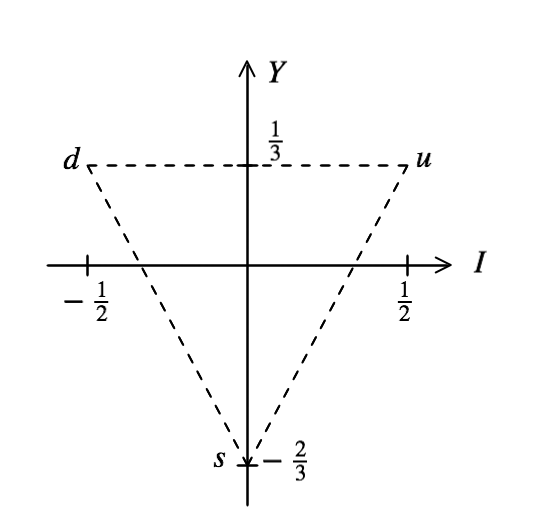
\includegraphics[width=0.5\textwidth]{images/web_feynman/image_47.png}
    \caption[Isospin and weak hypercharge of the $u$, $d$, and $s$ quarks]{Isospin and weak hypercharge of the $u$, $d$, and $s$ quarks.}
    \label{fig:ch12_IY_uds}
  \end{center}
\end{figure}

$f_{ijk}$ is an object with $8 \times 8 \times 8 = 512$ elements.  However there are only $9$ non-zero indepdendent values:

\begin{eqnarray*}
  f_{123} & = 1 & \\
  f_{132} & = -1 & \textrm{ etc} \\
  f_{458} & = f_{678} & = \frac{\sqrt{3}}{2} \\
  f_{147} & = f_{165} & = f_{246} \\
  & = f_{257} & = f_{345} \\
  & = f_{376} & = \frac{1}{2}
\end{eqnarray*}
\end{enumerate}

\section{Charged current interactions}

The theory concerning couplings and cross-sections of the charged current weak interactions can be extended to apply to quarks.

\begin{figure}[!htb]
  \begin{center}
    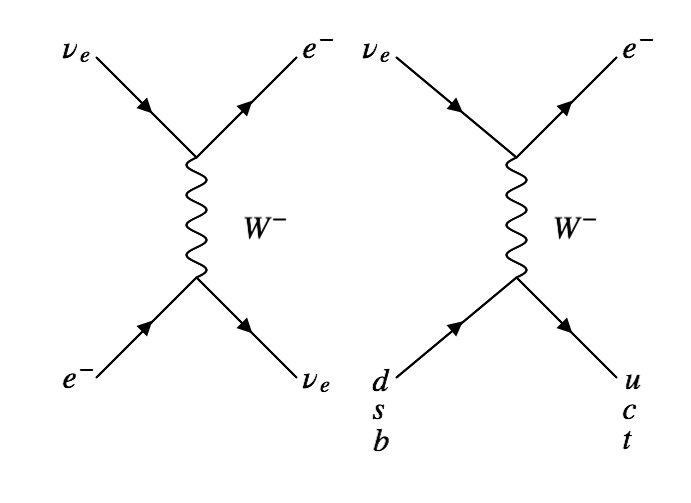
\includegraphics[width=0.75\textwidth]{images/web_feynman/image_48.png}
    \caption[Charged current interactions with quarks]{Charged current interactions with quarks.}
    \label{fig:ch12_chargedCurrentQuarks}
  \end{center}
\end{figure}

Going back to to when only $u$, $d$ and $s$ quarks were known it had already become apparent that the weak eigenstates are not the same as the mass eigenstates.  Cabibbo in 1963 proposed the following theory:

\[
  \left(
  \begin{array}{c}
    d' \\
    s'
  \end{array}
  \right)
  =
  \left(
  \begin{array}{cc}
    \cos\theta_c  & \sin\theta_c \\
    -\sin\theta_c & \cos\theta_c
  \end{array}
  \right)
  \left(
  \begin{array}{c}
    d \\
    s
  \end{array}
  \right)
\]

where the weak eigenstates are $d'$, $s'$ and the mass eigenstates are $d$, $s$.

For this theory to make sense the $d$ and $s$ masses have to be different.  $\theta_c$ is the Cabibbo angle and is $\sim 17^{\circ}$ and its origin is still a mystery, although there is some insight from the Higgs mechanism.

There must be a weak current which couples eg a $u$ quark to an $\bar{s}$ quark.  Instead of introducing a new coupling, it is assumed that the charged current couples rotated quark states.

It is now known that the form of the charged current weak interaction for two generations is of the form:

\[
  \left(\bar{u} \quad \bar{c}\right)\gamma_{\mu}\left(1 - \gamma^5\right)
  \left(
  \begin{array}{cc}
    \cos\theta_c  & \sin\theta_c \\
    -\sin\theta_c & \cos\theta_c
  \end{array}
  \right)
  \left(
  \begin{array}{c}
    d \\
    s
  \end{array}
  \right)
\]

The Cabibbo theory with one angle would have been valid had their only been four quarks.  However it is now known that there is another generation so the theory needs to be extended:

\[
  \left(\bar{u}\quad\bar{c}\quad\bar{t}\right)\gamma_{\mu}\left(1 - \gamma^5\right)V
  \left(
  \begin{array}{c}
    d \\
    s \\
    b
  \end{array}
  \right)
\]

where $V$ is the CKM matrix and is unitary.

This is now the form of the charged current interaction for quarks.

$V$ is generally seen written as:

\[
  V =
  \left(
  \begin{array}{ccc}
    V_{ud} & V_{us} & V_{ub} \\
    V_{cd} & V_{cs} & V_{cb} \\
    V_{td} & V_{ts} & V_{tb}
  \end{array}
  \right)
\]

where $V_{ud} \sim V_{cs} \sim V_{tb} \sim 1$ and the other values are small ($< 0.2$).

For this matrix there are $n^2 = 9$ elements, but since a unitary matrix is an orthogonal matrix there are $\frac{n(n-1)}{2}=3$ independent elements (or mixing angles).  Of the remaining $6$ parameterers, $5$ can be absorbed into arbitrary phase rotations of the quark fields, so there is $1$ independent phase.

The standard parameterisation is:

\[
  V = 
  \left(
  \begin{array}{ccc}
    \cos\theta_{12}\cos\theta_{13} & \sin\theta_{12}\cos\theta_{13} & \sin\theta_{13}\e^{-i\delta} \\
    &&\\
    -\sin\theta_{12}\cos\theta_{23} -  & \cos\theta_{12}\cos\theta_{23} - & \sin\theta_{23}\cos\theta_{13} \\
    \cos\theta_{12}\sin\theta_{23}\sin\theta_{13}\e^{i\delta} & \sin\theta_{12}\sin\theta_{13}\sin\theta_{23}\e^{i\delta} & \\
    &&\\
    \sin\theta_{12}\sin\theta_{23} - & -\cos\theta_{12}\cos\theta_{23} - & \cos\theta_{23}\cos\theta_{13} \\
    \cos\theta_{12}\sin\theta_{23}\sin\theta_{13}\e^{i\delta} & \sin\theta_{12}\sin\theta_{13}\sin\theta_{23}\e^{i\delta} &\\
  \end{array}
  \right)
\]

The phase $\e^{i\delta}$ is responsible for $CP$ violation.  However, even if $\delta$ was at its maximum possible value this would not be enough to explain why matter dominates over antimatter in the universe.

In the early 1970s, before charm quarks had been discovered the form of the charged current was expressed as:

\[
  \left(\bar{u} \quad \bar{c}\right)
  \left(
  \begin{array}{cc}
    \cos\theta_c  & \sin\theta_c \\
    -\sin\theta_c & \cos\theta_c
  \end{array}
  \right)
  \left(
  \begin{array}{c}
    d \\
    s
  \end{array}
  \right)
\]

Glashow, Iliopoulos and Maiani (GIM) proposed the existence of the $c$ quark before its discovery.  The existence and mass were predicted by using measurements of the weak decay of the $K^0 \to \mu^+ \mu^-$.

\begin{figure}[!htb]
  \begin{center}
    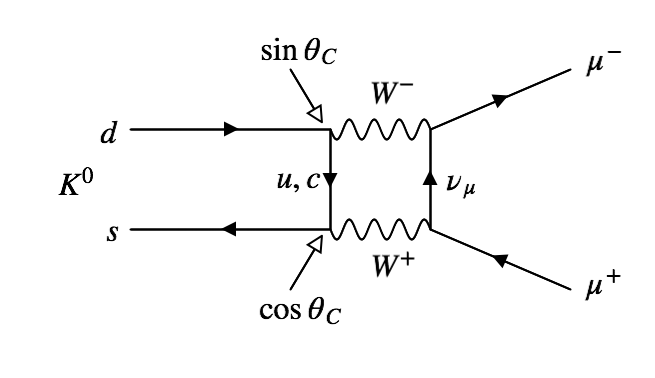
\includegraphics[width=0.75\textwidth]{images/web_feynman/image_49.png}
    \caption[$K^0\to\mu\mu$ decay]{$K^0\to\mu\mu$ decay.  Rate $\propto \cos\theta_c\sin\theta_c$}
    \label{fig:ch12_K0ToMuMu}
  \end{center}
\end{figure}

The predicted rate of the $K_0$ decay is $R$:

\[
  R = \frac{K^0 \to \mu^+\mu^-}{K^0 \to \textrm{all modes}}
\]

was higher than that observed.  This was solved by GIM, where they predicted an additional diagram.

The rate via the $c$ quark is: $Rate \propto -\cos\theta_c\sin\theta_c$

If the $u$ and $c$ masses had been the same then the two diagrams would have cancelled, so using the measured rate, the $c$ quark's existence could be postulated and its mass also predicted.  The $c$ quark was discovered soon after.

A classic example of a preferential is the decay of the $D^+$ which is $c\bar{d}$.  The favoured decay is $c \to s \quad u \quad \bar{d}$

\begin{figure}[!htb]
  \begin{center}
    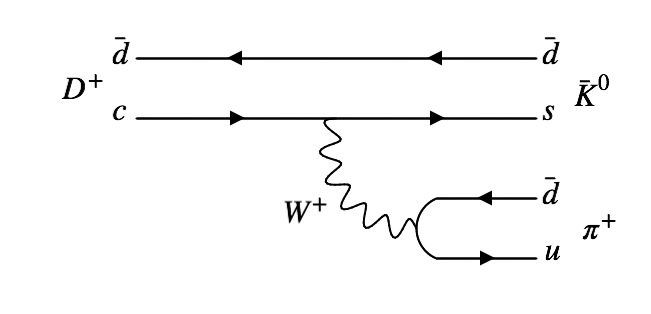
\includegraphics[width=0.75\textwidth]{images/web_feynman/image_50.png}
    \caption[$D^+\to\bar{K}^0\pi^+$ decay]{$D^+\to\bar{K}^0\pi^+$ decay.}
    \label{fig:ch12_DToK0Pi}
  \end{center}
\end{figure}

\[
  Rate \propto \cos^2\theta_c
\]

So a $\bar{K}$ meson is produced.  However for $D^+ \to K$, the rate is $R \propto \sin\theta_c$ and as $\cos^2\theta_c >> \sin^2\theta_c$ the mode $K^- \pi^+ \pi^+$ is highly favoured over $K^+ \pi^+ \pi^-$.

\clearpage

\section{Neutrino quark scattering}

Having previously calculated the weak current and cross-section for $\nu_{\e} \quad \e^-$, these results can be used to state the neutrino-quark cross-section.  Of course there are no colliders with a $\nu$ beam and lone quarks.  Quarks are always confined to hadrons and these experiments are known as deep inelastic scattering experiments.

The diagram for deep inelsatic scatting is:

\begin{figure}[!htb]
  \begin{center}
    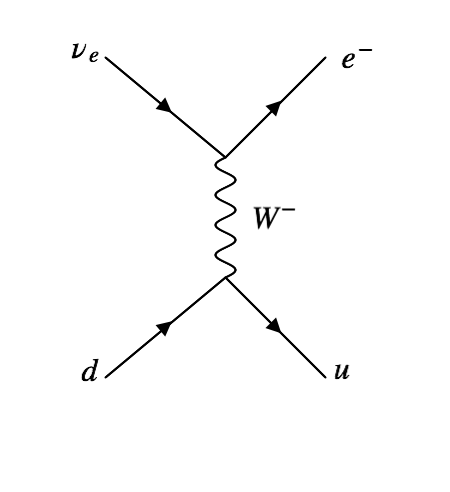
\includegraphics[width=0.4\textwidth]{images/web_feynman/image_51.png}
    \caption[Deep inelastic scattering]{Deep inelastic scattering.}
    \label{fig:ch12_DIS}
  \end{center}
\end{figure}

The weak current is constructed for quarks just as it is for leptons.

So the process goes from that shown in figure \ref{fig:ch12_WENu} to that shown in figure \ref{fig:ch12_WQQ}.

\begin{figure}[!htb]
  \begin{center}
    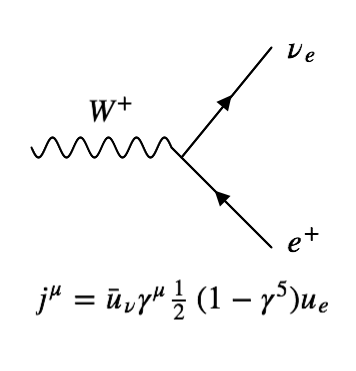
\includegraphics[width=0.4\textwidth]{images/web_feynman/image_52.png}
    \caption[Born level $W\to e\nu_e$]{Born level $W\to e\nu_e$.}
    \label{fig:ch12_WENu}
  \end{center}
\end{figure}

\begin{figure}[!htb]
  \begin{center}
    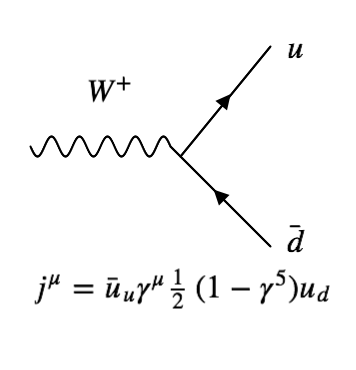
\includegraphics[width=0.4\textwidth]{images/web_feynman/image_53.png}
    \caption[Born level $W\to q\bar{q'}$]{Born level $W\to q\bar{q'}$.}
    \label{fig:ch12_WQQ}
  \end{center}
\end{figure}

Therefore the same procedure as before leads to:

\[
  \frac{\mathrm{d}\sigma}{\mathrm{d}\Omega}\left(\nu_{\e} \quad d \to \e^- \quad u\right) = \frac{G_F^2s}{4\pi^2} = \frac{\mathrm{d}\sigma}{\mathrm{d}\Omega}\left(\bar{\nu}_{\e}\bar{d}\right)
\]

and

\[
  \frac{\mathrm{d}\sigma}{\mathrm{d}\Omega}\left(\bar{\nu}_{\e}\quad u \to \e^+\quad d\right) = \frac{G_F^2s}{16\pi^2}\left(1 + \cos\theta\right)^2 = \frac{\mathrm{d}\sigma}{\mathrm{d}\Omega}\left(\nu_{\e}\bar{u}\right)
\]

where $\theta$ is the centre of mass system scattering angle.

The form of the cross-section is also often written as:

\begin{eqnarray*}
  \frac{\mathrm{d}\sigma}{\mathrm{d}\Omega}\left(\bar{\nu}_{\e} u\right) & = & \frac{G_F^2s}{4\pi^2}\left(1 - y\right)^2 \\
  \textrm{where } 1 - y & \simeq & \frac{1}{2}\left(1 + \cos\theta\right)
\end{eqnarray*}

$y$ is one of the DIS variables called the inelasticity.

\section{\texorpdfstring{$\pi/K$}{PiK} decays}

Consider the decays of the charged pions and kaons:

\[
  \pi^- / K^- \to \e^-/\mu^- \quad \bar{\nu}_{\e} / \bar{\nu}_{\mu}
\]

There are four possible combinations, as shown in figure \ref{fig:ch12_PiKToENuMuNu}:

\begin{figure}[!htb]
  \begin{center}
    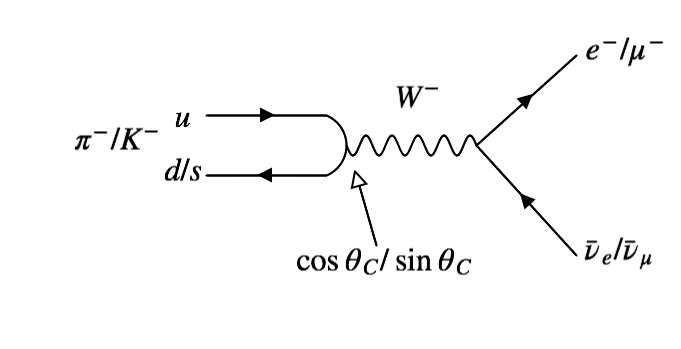
\includegraphics[width=0.8\textwidth]{images/web_feynman/image_54.png}
    \caption[Decay of $K/\pi\to e\nu_e/\mu\nu_\mu$]{Decay of $K/\pi\to e\nu_e/\mu\nu_\mu$.}
    \label{fig:ch12_PiKToENuMuNu}
  \end{center}
\end{figure}

For $\pi^- \to \mu^- \quad \bar{\nu}_{\mu}$ the four-momenta are:

\begin{eqnarray*}
  \pi^-(q) & \to & \mu^-(p) \quad \bar{\nu}_{\mu}(k) \\
  q & = & p + k \\
  \Rightarrow T_{fi} & = & \frac{G_F}{\sqrt{2}}f_{\pi}\cos\theta_c q_{\mu}\bar{u}(p)\gamma^{\mu}\left(1 - \gamma^5\right)v(k)
\end{eqnarray*}

There are many terms in this transition amplitude.  In a naive treatment it could be thought that the $W-$quark vertex could be written as $\bar{u_d}\gamma^{\mu}\left(1 - \gamma^5\right)\nu_{\bar{u}}$, but this is incorrect as the quarks are in bound states and not free.  The mesnon's four-momentum $q^{\mu}$ us the only four-vector available and $f_{\pi}$ is a function of $q^2$, but $q^2 = m^2_{\pi}$, so $f_{\pi}$ is a constant.  This pion decay constant characterises the strong interaction probability of the $d \bar{u}$ process and should in principle be calculable in QCD.

To calculate $T_{fi}^{\star} = T_{fi}^{\dagger}$:

\begin{eqnarray*}
  T_{fi} & = & \frac{G_F}{\sqrt{2}}f_{\pi}\cos\theta_c\Big[\bar{u}(p)\left(p_{\mu}\gamma^{\mu} + k_{\mu}\gamma^{\mu}\right)\left(1 - \gamma^5\right)v(k)\Big] \\
  \textrm{Recall } \not{p}\bar{u} & = & m_{\mu}\bar{u} \\
  \textrm{and }\left(\not{k} + m\right) v & \simeq & \not{k}v = 0 \\
  \Rightarrow T_{fi} & = & \frac{G_F}{\sqrt{2}}f_{\pi}\cos\theta_c m_{\mu}\Big[\bar{u}(p)\left(1 - \gamma^5\right)v(k)\Big] \\
  \Rightarrow |T_{fi}|^2 & = & \frac{G_F^2}{2}\left(f_{\pi}\right)^2\cos^2\theta_c m^2_{\mu}Tr\Big[\left(\not{p} + m_{\mu}\right)\left(1 - \gamma^5\right)\not{k}\left(1 + \gamma^5\right)\Big] \\
  & = & 4G_F^2\left(f_{\pi}\right)^2\cos^2\theta_c m^2_{\mu}\left(p \cdot k \right)
\end{eqnarray*}

In the $\pi$ rest frame $\ul{k} = -\ul{p}$:

\begin{eqnarray*}
  \textrm{So } p \cdot k & = & EE' - \ul{k}\cdot\ul{p} \\
  & = & EE' + k^2 \\
  & = & EE' + \left(E'\right)^2
\end{eqnarray*}

The decay rate is given by:

\begin{eqnarray*}
  \mathrm{d}\Gamma & = & \frac{1}{2m_{\pi}}|T_{fi}|^2\frac{\mathrm{d}^3p}{\left(2\pi\right)^2}\frac{1}{2E} \frac{\mathrm{d}^3k}{\left(2\pi\right)^2}\frac{1}{2E'}\left(2\pi\right)^4\delta^4\left(q - p - k\right) \\
  \Rightarrow \Gamma & = & \frac{G_F^2\left(f_{\pi}\right)^2\cos^2\theta_cm^2_{\mu}}{\left(2\pi\right)^2 2m_{\pi}}\int\frac{\mathrm{d}^3p\mathrm{d}^3k}{EE'}\delta\left(m_{\pi} - E - E'\right)\delta^3\left(\ul{k} + \ul{p}\right)E'\left(E + E'\right)
\end{eqnarray*}

$\mathrm{d}^3p$ integration acts on the $\delta^3$ function.  As there is no angular dependence, $\mathrm{d}\Omega \to 4\pi$ and the integration is over $E'$.

\begin{eqnarray*}
  \Rightarrow \Gamma & = & \frac{G_F^2\left(f_{\pi}\right)^2\cos^2\theta_c m^2_{\mu}}{\left(2\pi\right)^2 2m_{\pi}}4\pi\int\mathrm{d}E' E'^{2}\left(1 + \frac{E'}{E}\right)\delta\left(m_{\pi} - E - E'\right) \\
  \textrm{but } \delta\Big[f\left(E'\right)\Big] & = & \frac{\delta\left(E' - E'_0\right)}{\left.\frac{\partial f}{\partial E}\right|_{E' - E'_0}} \\
  & = & \frac{\delta\left(E' - E'_0\right)}{1 + \frac{E'_0}{E}} \\
  \textrm{and } E & = & \sqrt{m^2_{\mu} + E'^2} \\
  \textrm{where } E'_0 & = & \frac{m^2_{\pi} - m^2_{\mu}}{2m_{\pi}}
\end{eqnarray*}

The result of the integration over $E_0^2$ is:

\[
  \Gamma = \frac{G_F^2}{8\pi^2}\left(f_{\pi}\right)^2\cos^2\theta_c m^2_{\mu}m_{\pi}\left(1 - \frac{m^2_{\mu}}{m^2_{\pi}}\right)^2
\]

For the decay to an electron substitute $m_{\mu} \to m_{\e}$ and for the decay of kaons use the substitutions $\cos^2\theta_c \to \sin^2\theta_c$ and $m_{\pi} \to m_K$.

The ratio of $\mu/\e$ decay rates is:

\begin{eqnarray*}
  R & = & \frac{\Gamma\left(\pi^- \to \e^- \quad \bar{\nu}_{\e}\right)}{\Gamma\left(\pi^- \to \mu^- \quad \bar{\nu}_{\mu}\right)} \\
  & = &
  \left(\frac{m_{\e}}{m_{\mu}}\right)^2\left(\frac{m^2_{\pi} - m^2_{\e}}{m^2_{\pi} - m^2_{\mu}}\right)^2 \\
  & = & 1.28 \times 10^{-4}
\end{eqnarray*}

Therefore the decay to muons is strongly favoured over the decay to electrons.  This is understood by considering angular momentum.  In the decay the antineutrino is expected to have helicity $+1$ and as the $\pi$ has helicity $0$, then the helicity of the electron is also $1$.  However, as $m_{\e}\to 0$ the helicity of the electron should tend to $-1$.  So the electron is forced into a non-preferential helicity state, hence the suppression is related to the ratio of the masses squared.

\section{Width of the \texorpdfstring{$W^{\pm}$}{Wpm}}

An ``exact'' first order calculation , assuming the masses of the neutrinos and $\bar{s}/\bar{d}$ quarks are zero gives the possible decay channels of the $W$ as:

\begin{eqnarray*}
  W^{\pm} & \to & \e^+ \quad \nu_{\e} \\
  & \to & \mu^+ \quad \nu_{\mu} \\
  & \to & \tau^+ \quad \nu_{\tau} \\
  & \to & u \quad \bar{d}/\bar{s} \\
  & \to & c \quad \bar{d}/\bar{s} \\
  & \to & \left( t \quad \bar{b}\right)
\end{eqnarray*}

\begin{figure}[!htb]
  \begin{center}
    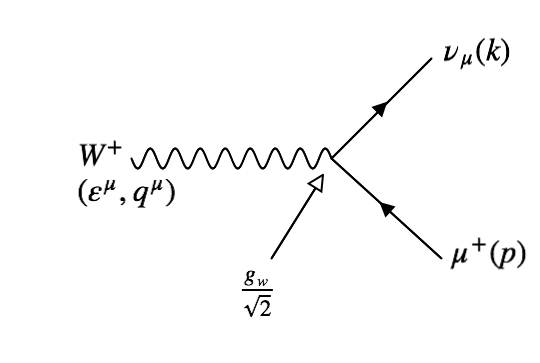
\includegraphics[width=0.8\textwidth]{images/web_feynman/image_55.png}
    \caption[Decay of $W\to\mu\nu_\mu$]{Decay of $W\to\mu\nu_\mu$.}
    \label{fig:ch12_WMuNu}
  \end{center}
\end{figure}

\begin{eqnarray*}
  T_{fi} & = & \frac{g_W}{\sqrt{2}}\epsilon^{\mu}\bar{u}(k)\gamma_{\mu}\frac{1}{2}\left(1 - \gamma^5\right)v(p) \\
  |T_{fi}|^2 & = & \frac{1}{3}\frac{g_W^2}{2}\sum\epsilon^{\mu}\epsilon^{\nu \star}\Big[\bar{v}(p)\gamma^{\nu}\frac{1}{2}\left(1 - \gamma^5\right)u(k)\Big]\Big[\bar{u}(k)\gamma^{\mu}\frac{1}{2}\left(1 - \gamma^5\right)v(p)\Big] \\
  & = & \frac{1}{3}\frac{g_W^2}{2}\Big[ -g^{\mu\nu} + \frac{q^{\mu}q^{\nu}}{M^2_W}\Big]Tr\Big[\left(\not{p} - \not{m_{\mu}}\right)\gamma^{\nu}\frac{1}{2}\left(1 - \gamma^5\right)\not{k}\gamma^{\mu}\frac{1}{2}\left(1 - \gamma^5\right)\Big]
\end{eqnarray*}

$m_{\mu}$ does not contribute as it multiplies $3\gamma$ matrices.  The factor of $\frac{1}{3}$ is due to the $3$ polarisation states of the $W$ boson.

\begin{eqnarray*}
  |T_{fi}|^2 & = & \frac{1}{3}\frac{g^2_W}{2\times 2}\left(-g^{\mu\nu} + \frac{q^{\mu}q^{\nu}}{M^2_W}\right) Tr\Big[(\not{p}\gamma^{\nu}\not{k}\gamma^{\mu}\left(1 - \gamma^5\right)\Big] \\
  & = & \frac{g^2_W}{3}\left(-g^{\mu\nu} + \frac{q^{\mu}q^{\nu}}{M^2_W}\right)\left(p_{\mu}k_{\nu} + p_{\nu}k_{\mu} - g_{\mu\nu}p\cdot k\right)
\end{eqnarray*}

The $\gamma^5$ term gives an antisymmetric tensor which gives zero contribution when summed with the symmetric term.

\[
  |T_{fi}|^2 = \frac{g^2_W}{3}\left(p\cdot k + \frac{2\left(q\cdot k\right)\left(q\cdot p\right)}{M^2_W}\right)
\]

In the $W$ rest frame:

\begin{eqnarray*}
  q\cdot k & = & \frac{M^2_W}{2}\left(1 - \frac{m^2_{\mu}}{M^2_W}\right) \\
  q\cdot p & = & \frac{M^2_W}{2}\left(1 + \frac{m^2_{\mu}}{M^2_W}\right) \\
  |T_{fi}|^2 & = & \frac{g^2_W}{3}M^2_W\left(1 - \frac{m^2_{\mu}}{M^2_W}\right)\left(1 + \frac{m^2_{\mu}}{M^2_W}\right) \\
  \Rightarrow \Gamma & = & \frac{g^2_W}{48\pi}M_W \left(1 - \frac{m^2_{\mu}}{M^2_W}\right)\left(1 + \frac{m^2_{\mu}}{M^2_W}\right) \\
  & = & 0.227 \gev \\
  \Rightarrow \Gamma_T & = & N_l \Gamma_{l\nu} + N_{colour}N_q\Gamma_{l\nu} \\
  & = & \left(3 + 3\times2\right)\Gamma \\
  & = & 9\Gamma \\
  & = & 2.05 \gev
\end{eqnarray*}

The measured value (from the PDG) is $2.141 \pm 0.041 \gev$ which is in good agreement to the first order.
